\documentclass{standalone}
\usepackage{tikz}

\begin{document}

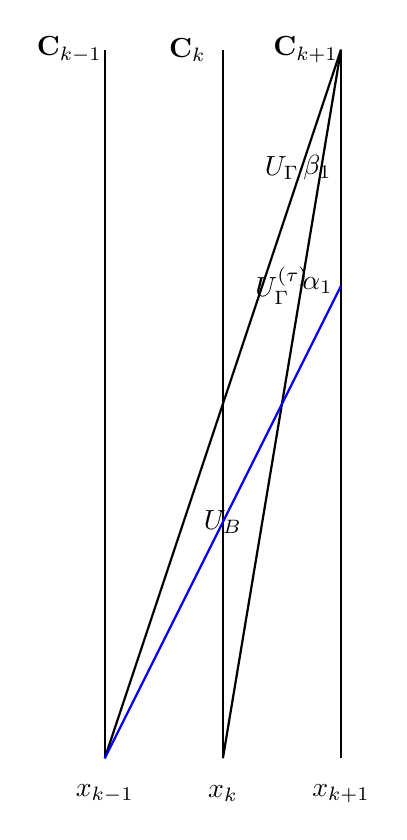
\begin{tikzpicture}[scale=1.5]
    % Draw vertical lines
    \draw[thick] (0,0) -- (0,6);
    \draw[thick] (1,0) -- (1,6);
    \draw[thick] (2,0) -- (2,6);
    
    % Label points
    \node at (-0.3, 6) {$\mathbf{C}_{k-1}$};
    \node at (0.7, 6) {$\mathbf{C}_k$};
    \node at (1.7, 6) {$\mathbf{C}_{k+1}$};
    \node at (0, -0.3) {$x_{k-1}$};
    \node at (1, -0.3) {$x_k$};
    \node at (2, -0.3) {$x_{k+1}$};
    
    % Draw diagonal lines
    \draw[thick] (0,0) -- (2,6);
    \draw[thick] (1,0) -- (2,6);
    
    % Label angles
    \node at (1.8, 4) {$\alpha_1$};
    \node at (1.8, 5) {$\beta_1$};
    
    % Draw blue line
    \draw[blue, thick] (0,0) -- (2,4);
    
    % Label U_B
    \node at (1, 2) {$U_B$};
    
    % Label U_Gamma
    \node at (1.5, 5) {$U_\Gamma$};
    \node at (1.5, 4) {$U_\Gamma^{(\tau)}$};
\end{tikzpicture}

\end{document}